%%%%%%%%%%%%%%%%%%%%% Chapter 18 %%%%%%%%%%%%%%%%%%%%%%%%%%%%%%%%%
% Multimodal Privacy: Cross-Modal Data Fusion
%%%%%%%%%%%%%%%%%%%%%%%%%%%%%%%%%%%%%%%%%%%%%%%%%%%%%%%%%%%%%%%%%
\motto{When AI sees, hears, and reads everything, the risk of leakage is no longer additive---it is exponential.}

\chapter{Multimodal Privacy: Cross-Modal Data Fusion}
\label{chap:multimodal_privacy}

\abstract{Modern AI systems increasingly integrate multiple data streams---text, images, audio, and sensors---to understand the world more holistically. However, this convergence leads to complex new privacy risks. This chapter explores the concept of cross-modal leakage, where sensitive information in one modality can be inferred from another through high-dimensional correlations. We analyze secure fusion architectures, comparing early and late fusion strategies, and introduce implementations for private cross-modal attention. Ensuring that multimodal systems remain trustworthy requires protecting not just each individual data stream, but the hidden interactions between them.}

\section{When AI Sees, Hears, and Reads Everything}
\label{sec:multimodal_convergence_ch16}

In the preceding chapters, we explored privacy defenses for single-modal AI: tabular data, decentralized Federated Learning, and Large Language Models. However, the next generation of AI is increasingly \textbf{multimodal}. Multimodal models combine disparate data sources---such as a patient's medical images, their verbal clinical notes, and their wearable sensor data---to provide more accurate and context-aware insights.

While this holistic view improves utility, it introduces a significant security challenge: Protecting each modality individually is necessary but not sufficient. We must also protect the interactions between modalities.

\section{Unique Risks in Multimodal Systems}
\label{sec:multimodal_risks_ch16}

The Trustworthy AI Architect must defend against two primary cross-modal threats:

\subsection{Cross-Modal Inference Attacks}
\label{subsec:cross_modal_inference_ch16}

An adversary may use the presence of one modality to infer sensitive information in another that was supposed to be hidden. For example, a model might be able to infer a patient's medical diagnosis (text) purely from the anatomical structure in their medical image, even if the text records were private. This risk can be quantified using the \textbf{Mutual Information} between modalities:
\begin{equation}
I(X_{\text{image}}; X_{\text{text}}) = \sum_{x_i, x_t} p(x_i, x_t) \log \frac{p(x_i, x_t)}{p(x_i) p(x_t)}
\end{equation}

\begin{figure}[t]
\centering
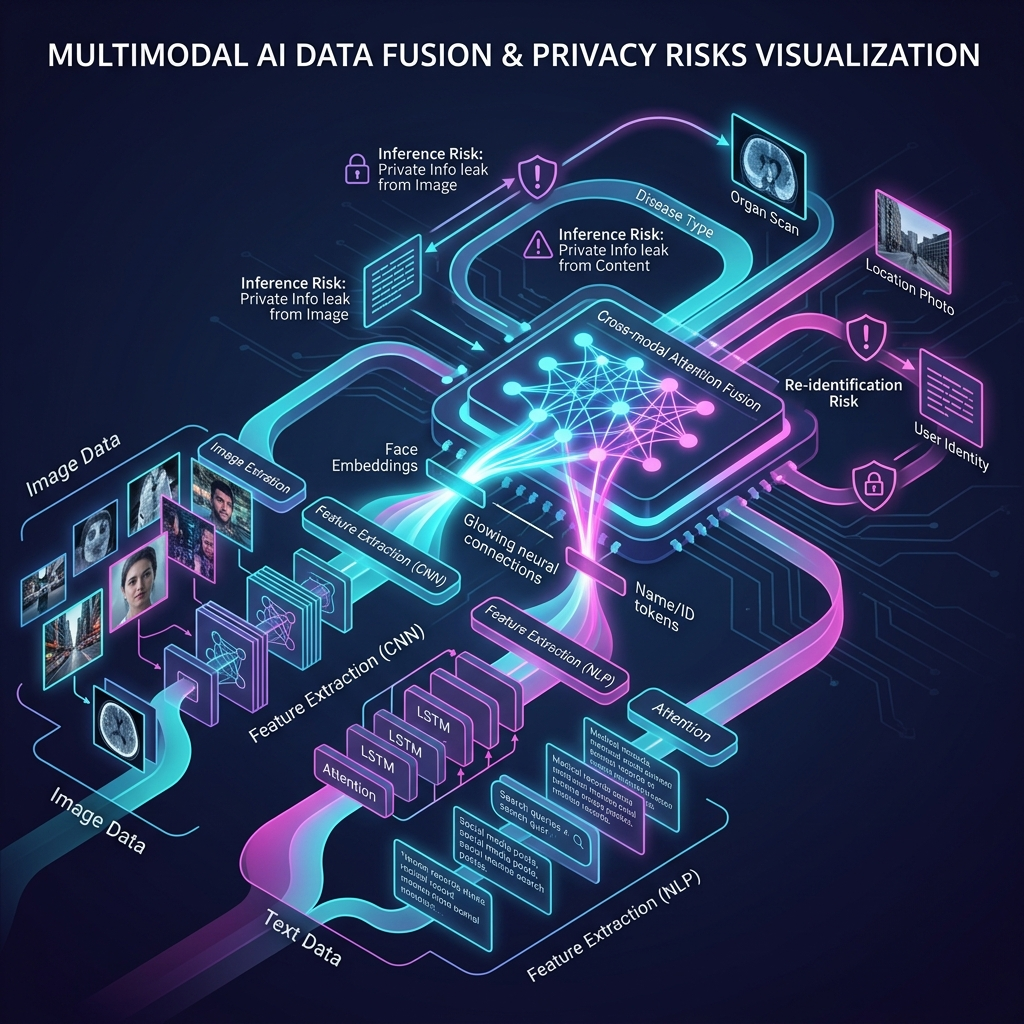
\includegraphics[width=0.9\textwidth]{figures/ch16_multimodal.png}
\caption{Multimodal AI Data Fusion and Privacy Risks: Visualizing how cross-modal attention can lead to the inference of sensitive data from seemingly unrelated modalities.}
\label{fig:ch16_multimodal}
\end{figure}

\subsection{Insecure Fusion Architectures}
\label{subsec:fusion_risks_ch16}

The way modalities are combined during training and inference significantly impacts the system's privacy profile.

\begin{table}
\caption{Privacy Risks of Multimodal Fusion Strategies}
\label{tab:fusion_strategies_ch16}
\begin{tabular}{p{3cm}p{4cm}p{3cm}}
\hline\noalign{\smallskip}
Fusion Type & Description & Privacy Risk \\
\noalign{\smallskip}\svhline\noalign{\smallskip}
Early Fusion & Concatenating raw features before processing. & High: All modalities exposed to a single model. \\
Late Fusion & Processing modalities separately and combining final outputs. & Medium: Intermediate representations may still leak. \\
Hybrid/Attention & Learning weighted interactions (cross-attention). & Variable: Attention weights can reveal specific correlations. \\
\noalign{\smallskip}\hline\noalign{\smallskip}
\end{tabular}
\end{table}

\section{Implementing Private Cross-Modal Attention}
\label{sec:private_attention_ch16}

To mitigate these risks, architects can implement \textbf{Modality Isolation}. This involves adding independent Differential Privacy (DP) noise to each data stream before they reach the fusion layer. Furthermore, by adding noise directly to the \textit{attention weights} during cross-modal processing, we can prevent the model from learning "too much" about the correlation between private modalities.

\section{Conclusion}
\label{sec:conclusion_multimodal_ch16}

Multimodal privacy requires a defense-in-depth approach that recognizes the model's ability to "fill in the gaps" between data sources. By implementing secure fusion and modality isolation, we can build systems that be both holistically intelligent and strictly private. As models become more pervasive and permanent, however, a new requirement emerges: the ability to "forget." In the next chapter, we close Part V by exploring the technical requirements of \textbf{Machine Unlearning}.


